\documentclass[ngerman]{beamer}
\usetheme{metropolis}

% use \cref instead of autoref, autoref does not work with beamer
\usepackage{cleveref}

\usepackage{appendixnumberbeamer}


% some imports from handout, probably dont need all but whatever
\usepackage[utf8]{inputenc}
\usepackage[T1]{fontenc}   
\usepackage{graphicx}       
\usepackage[german]{babel}
\usepackage{csquotes}     
\usepackage{eurosym}
\usepackage{float}
\usepackage{rotating}
\usepackage{blkarray}
\usepackage{amsmath}
\usepackage{amssymb}
\usepackage{gensymb}
\usepackage{amsthm}
\usepackage{listings}
\usepackage{caption}
\usepackage{subcaption}
\usepackage{interval}
\usepackage{textpos}
\usepackage[style=authoryear, backend=biber]{biblatex}
\addbibresource{references.bib}


% argmin command
\newcommand{\argmin}[1]{\underset{#1}{\operatorname{arg}\,\operatorname{min}}\;}
% command for euclidean norm
\newcommand{\norm}[1]{\lVert#1\rVert}
% command for lagrangian L (kind of handwritten L)
\newcommand{\Lagr}{\mathcal{L}}

% show current page number in footer
\setbeamertemplate{footline}[frame number]


% No navigation symbols at the slides' bottom
\beamertemplatenavigationsymbolsempty

% command for creating a frame with one full-slide image without caption
% first arg: frame title, second arg: path to img
\newcommand {\imageframe}[2] {
	\begin{frame}{#1}
		\begin{center}
			\begin{figure}
			\includegraphics[width=\textwidth,height=0.8\textheight,keepaspectratio]{#2}
		\end{figure}
		\end{center}
	\end{frame}
}



\title{Support Vector Machines}
\author{André Hopfgartner \& Matthias Rupp}
\institute{Vorarlberg University of Applied Sciences \\ \\ \\ \\ \\ \\ 
\includegraphics[width=0.35\textwidth]{assets/Logo-A3.png}}

\date{08.06.2021}

\begin{document}

\begin{frame}[plain]
    \maketitle
\end{frame}


\begin{frame}{Agenda}
	\setbeamertemplate{section in toc}[sections numbered]
	\tableofcontents[hideallsubsections]
\end{frame}


\section{Einführung}


\begin{frame}{Intuition}
	\emph{Ziel}: lineare Trennung zweier Klassen\\ \pause
	\emph{Wie?}: Definition einer (Hyper-) Ebene \\ \pause
	\emph{Nebenbedingung}: Möglichst großer freier Bereich\\ \pause
	
	\begin{center}
		\begin{figure}
			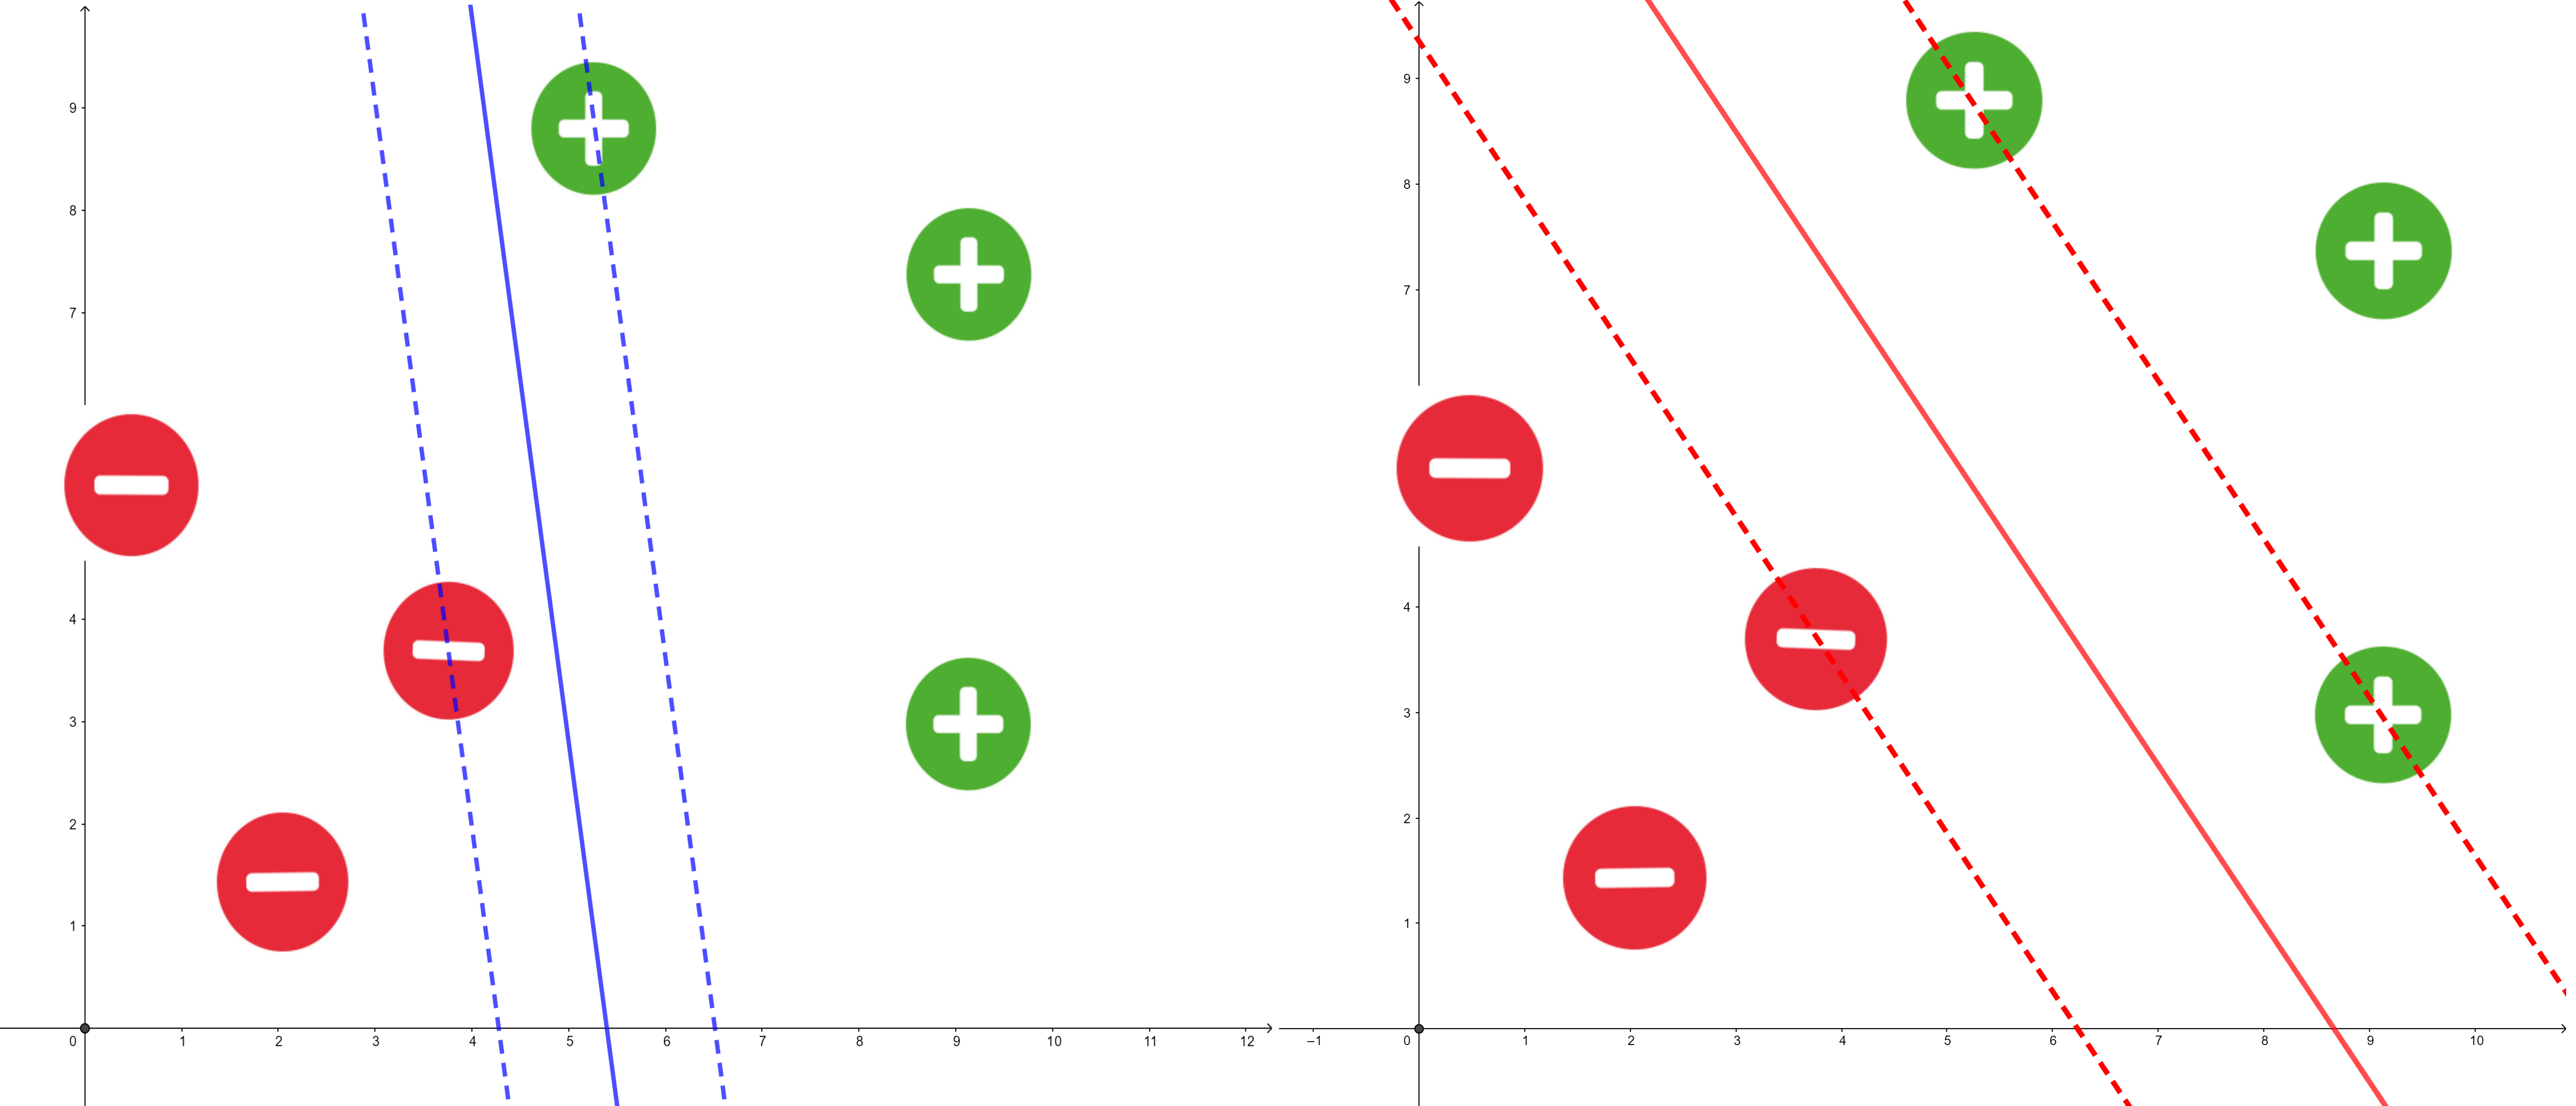
\includegraphics[width=\textwidth,height=0.7\textheight,keepaspectratio]{assets/small_vs_big_margin.png}
		\end{figure}
	\end{center}	
\end{frame}

\begin{frame}{Arten von SVM}
	\emph{Arten von SVM:}
	\begin{itemize}
		\item \emph{Hard-Margin SVM}: Daten werden 100\% korrekt getrennt
		\item \emph{Soft-Margin SVM}: Einzelne Datenpunkte können falsch klassifiziert werden um insgesamt bessere Trennung zu erhalten
	\end{itemize}

	\begin{center}
		\begin{figure}
			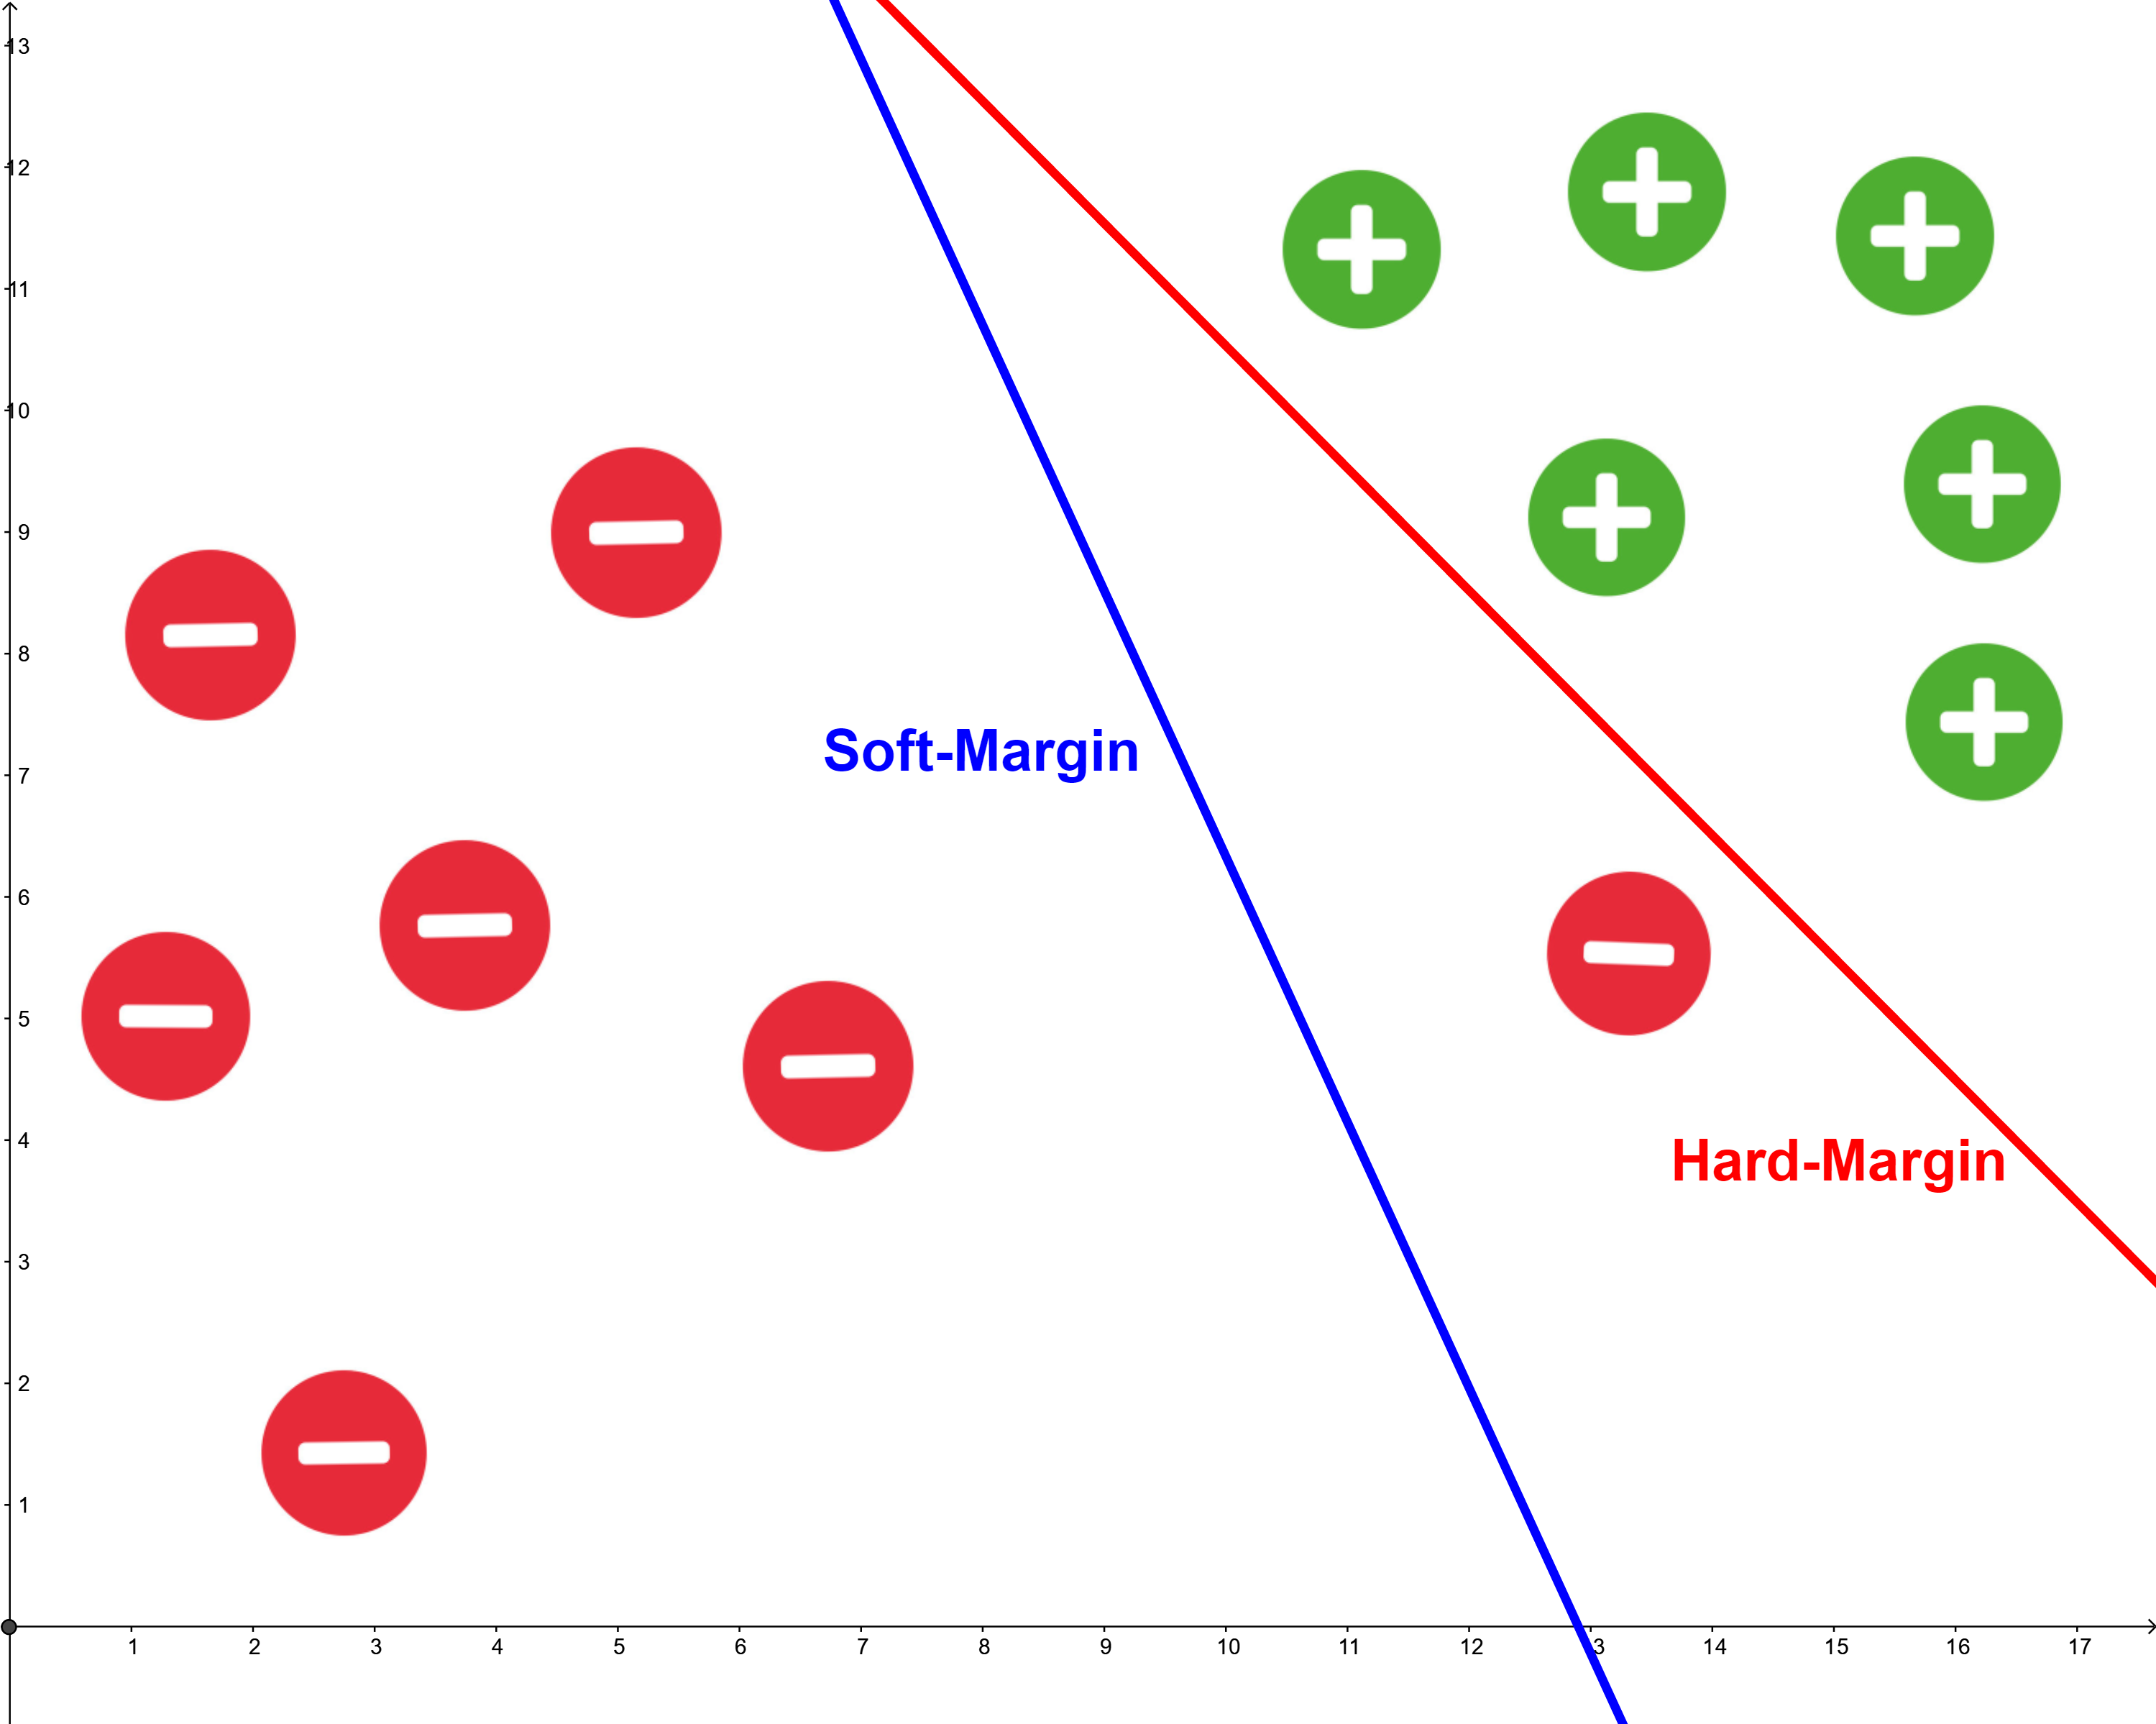
\includegraphics[width=\textwidth,height=0.6\textheight,keepaspectratio]{assets/hard_vs_soft_margin.png}
		\end{figure}
	\end{center}

\end{frame}

\section{Hard-Margin Support Vector Machine}


\begin{frame}{Mathematische Formulierung}
Gegeben sei ein Gewichtsvektor $w \in \mathbb{R}^{K}$, ein Bias $b \in \mathbb{R}$, ein beliebiger Punkt $x_{n} \in \mathbb{R}^{K}$ und ein zugehöriges Label $y_{n} \in \{-1, +1\}$. Eine Ebene im Raum kann allgemein definiert werden durch:

\begin{equation*} \label{plane_eq}
	\begin{aligned}
		w^{T} x_{n} + b &= 0 \\
	\end{aligned}
\end{equation*}

Ziel der SVM: $w$ und $b$ bestimmen für optimale Trennung

\end{frame}


\begin{frame}{Klassifikation}
	Annahme: $w$ und $b$ bereits bekannt\\
	Wie klassifiziert man einen Punkt $x_{n}$? \\ \pause
	Liegt $x_{n}$ über oder unter Ebene = Vorzeichen:
	\begin{subequations}
		\begin{alignat*}{2}
			y = sign(w^{T} x_{n} + b)  & \qquad & \text{ ist gleichbedeutend mit} \\
			w^{T} x_{n} + b > 0 & & \text{ für } y_{n} = +1\\
			w^{T} x_{n} + b < 0 & & \text{ für } y_{n} = -1
		\end{alignat*}
	\end{subequations}

	Bisher: Punkte können genau auf der Grenze liegen wenn $w^{T} x_{n} + b = 0$ \\
\end{frame}



\begin{frame}{Einführung eines Trennbandes}	
	Striktere Regel: Um Ebene soll Band frei bleiben \\
	\begin{subequations} \label{decision_rules}
		\begin{alignat*}{2}
			w^{T} x_{n} + b \geq +1 & \qquad & \text{ für } y_{n} = +1\\
			w^{T} x_{n} + b \leq -1 & & \text{ für } y_{n} = -1
		\end{alignat*}
	\end{subequations}

	\begin{center}
		\begin{figure}
			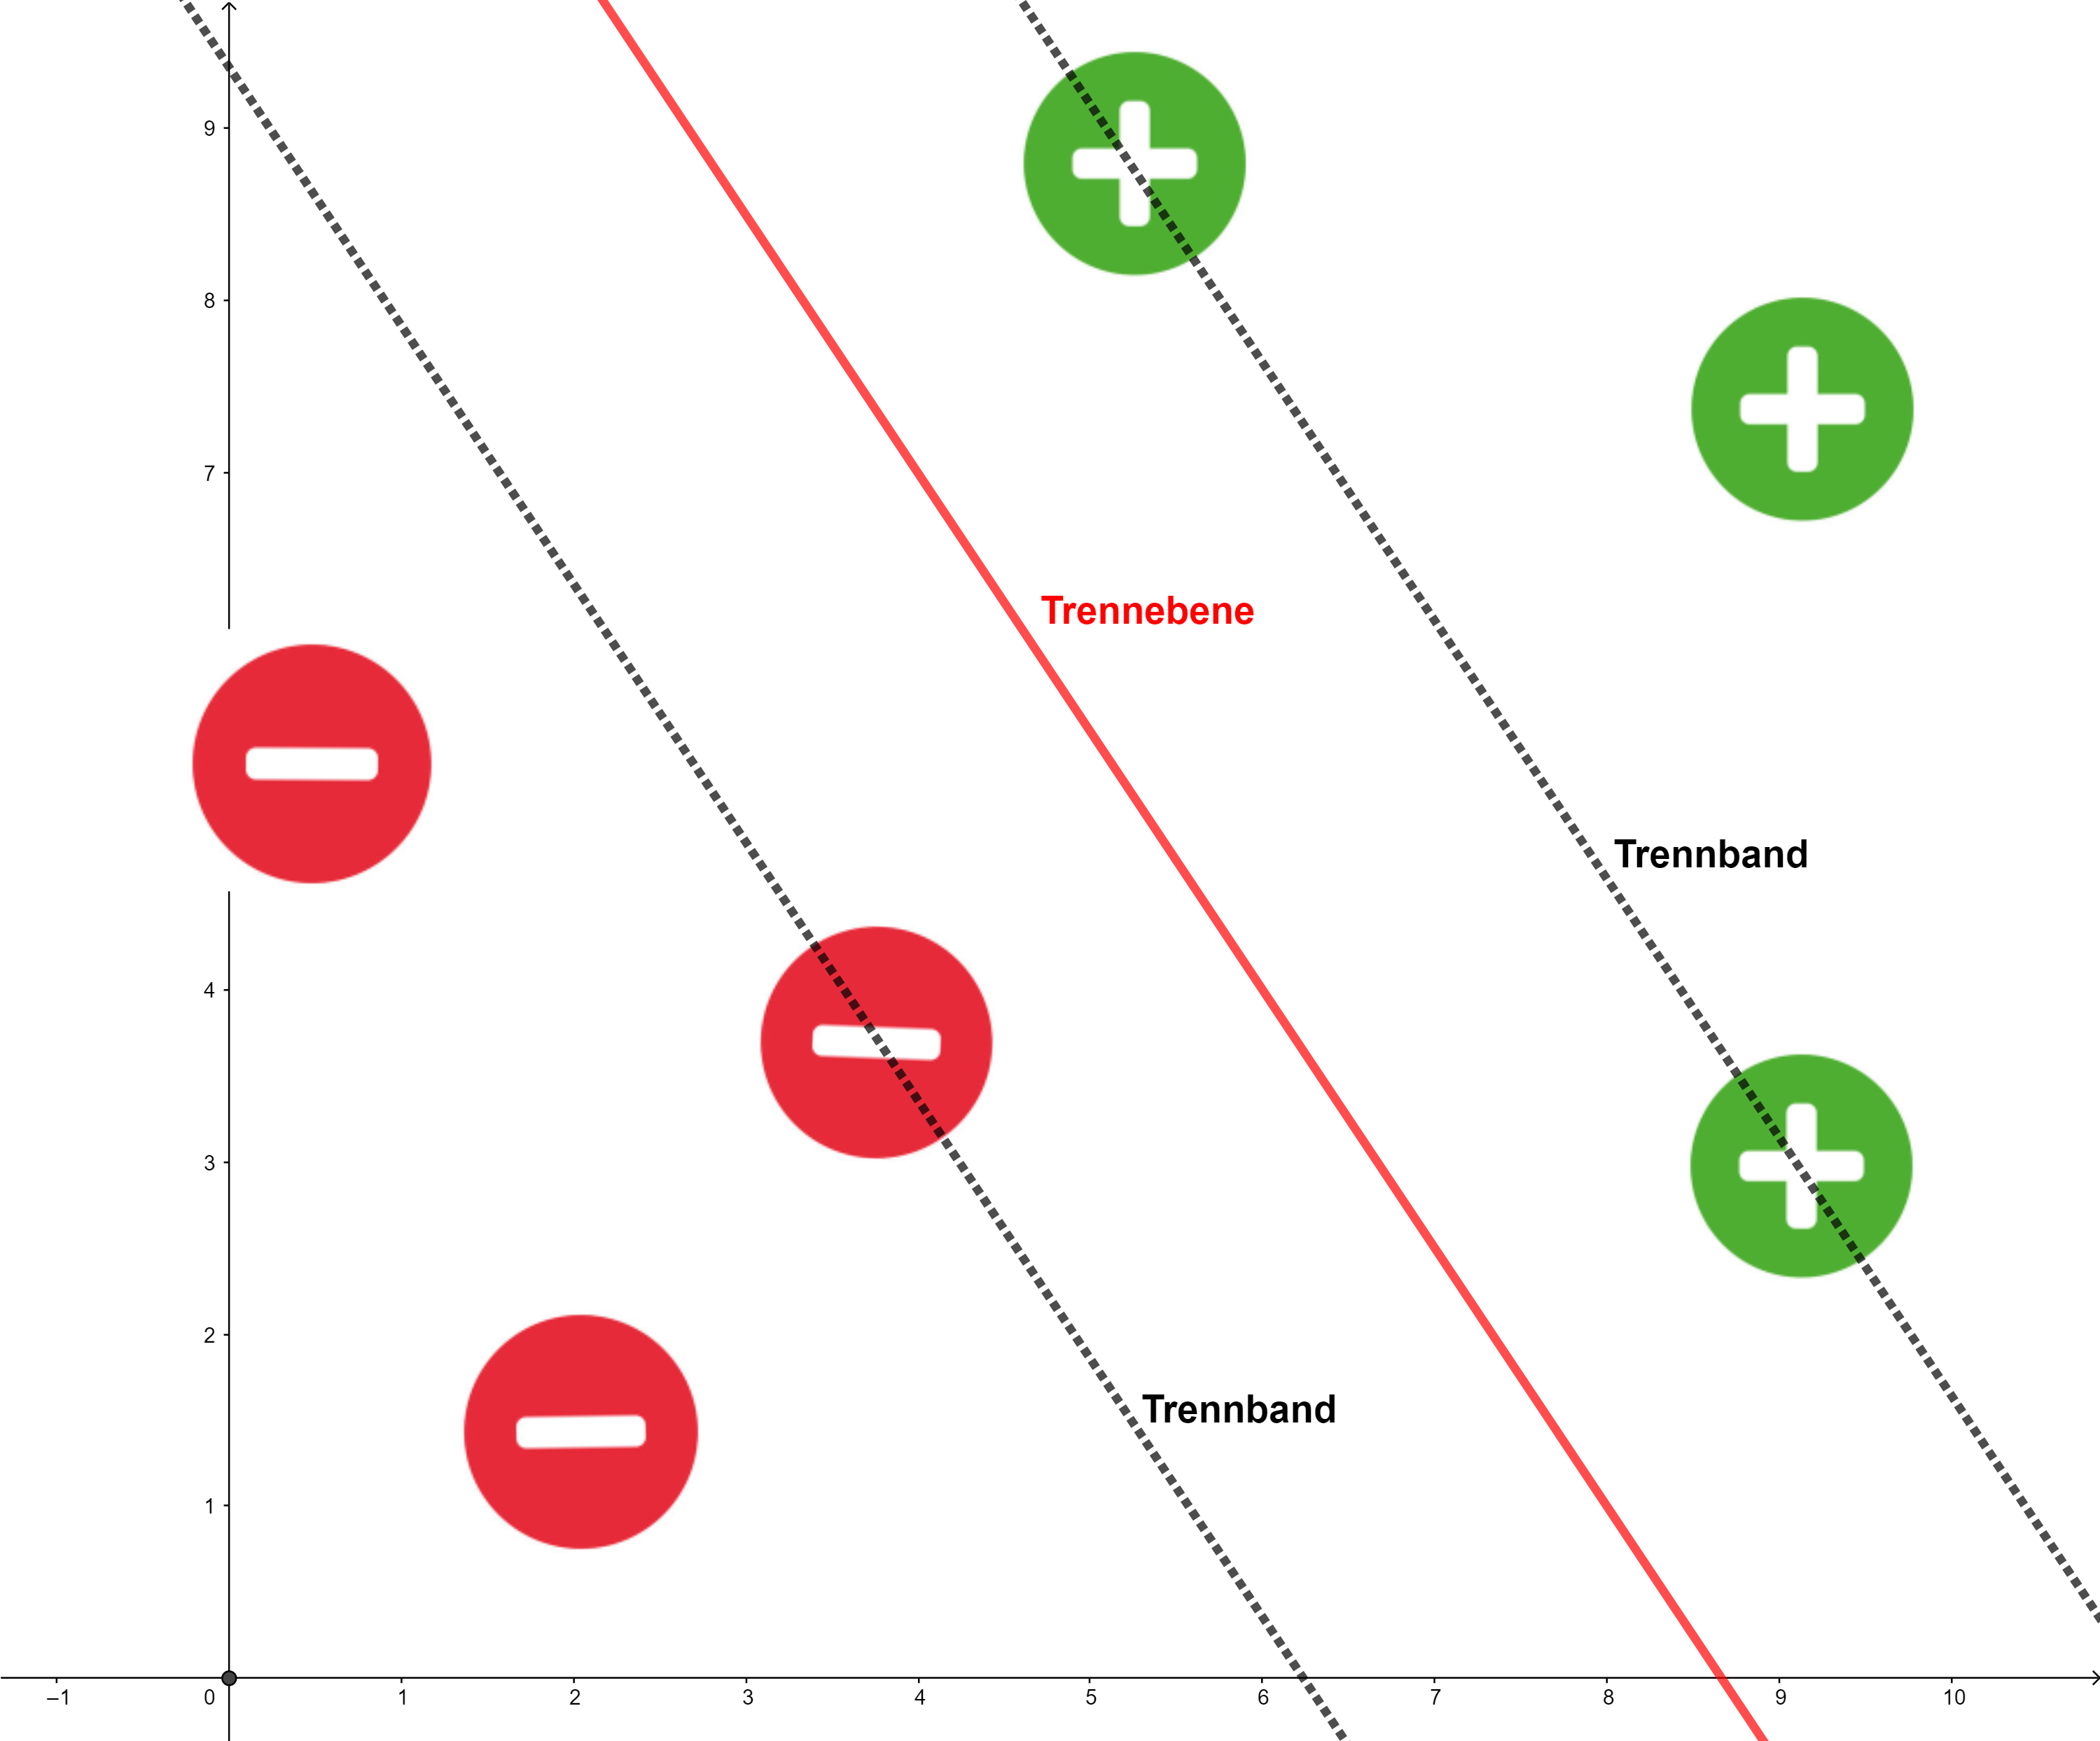
\includegraphics[width=\textwidth,height=0.6\textheight,keepaspectratio]{assets/trennband.png}
		\end{figure}
	\end{center}

\end{frame}

\begin{frame}{Einführung eines Trennbandes}
	Beidseitige Multiplikation mit $y_{n}$
	\begin{subequations}
		\begin{alignat*}{2}
			y_{n} (w^{T} x_{n} + b) \geq 1 & \qquad & \text{ für } y_{n} = +1\\
			y_{n} (w^{T} x_{n} + b) \geq 1 & & \text{ für } y_{n} = -1
		\end{alignat*}
	\end{subequations}

	\pause 
	Für den Fall, dass $x_{n} = \hat{x}$ genau an der Grenze des Trennbands liegt, gilt somit:
	\begin{equation*}
		\begin{aligned}
			y_{n} (w^{T} \hat{x} + b) &= 1
		\end{aligned}
	\end{equation*}
\end{frame}



\begin{frame}{Normalabstand eines Punktes zur Ebene}
	Gesucht: Normalabstand $d$ eines Punktes $x_{n} \in \mathbb{R}^{K}$ zur Ebene \\
	
	\begin{center}
		\begin{figure}
			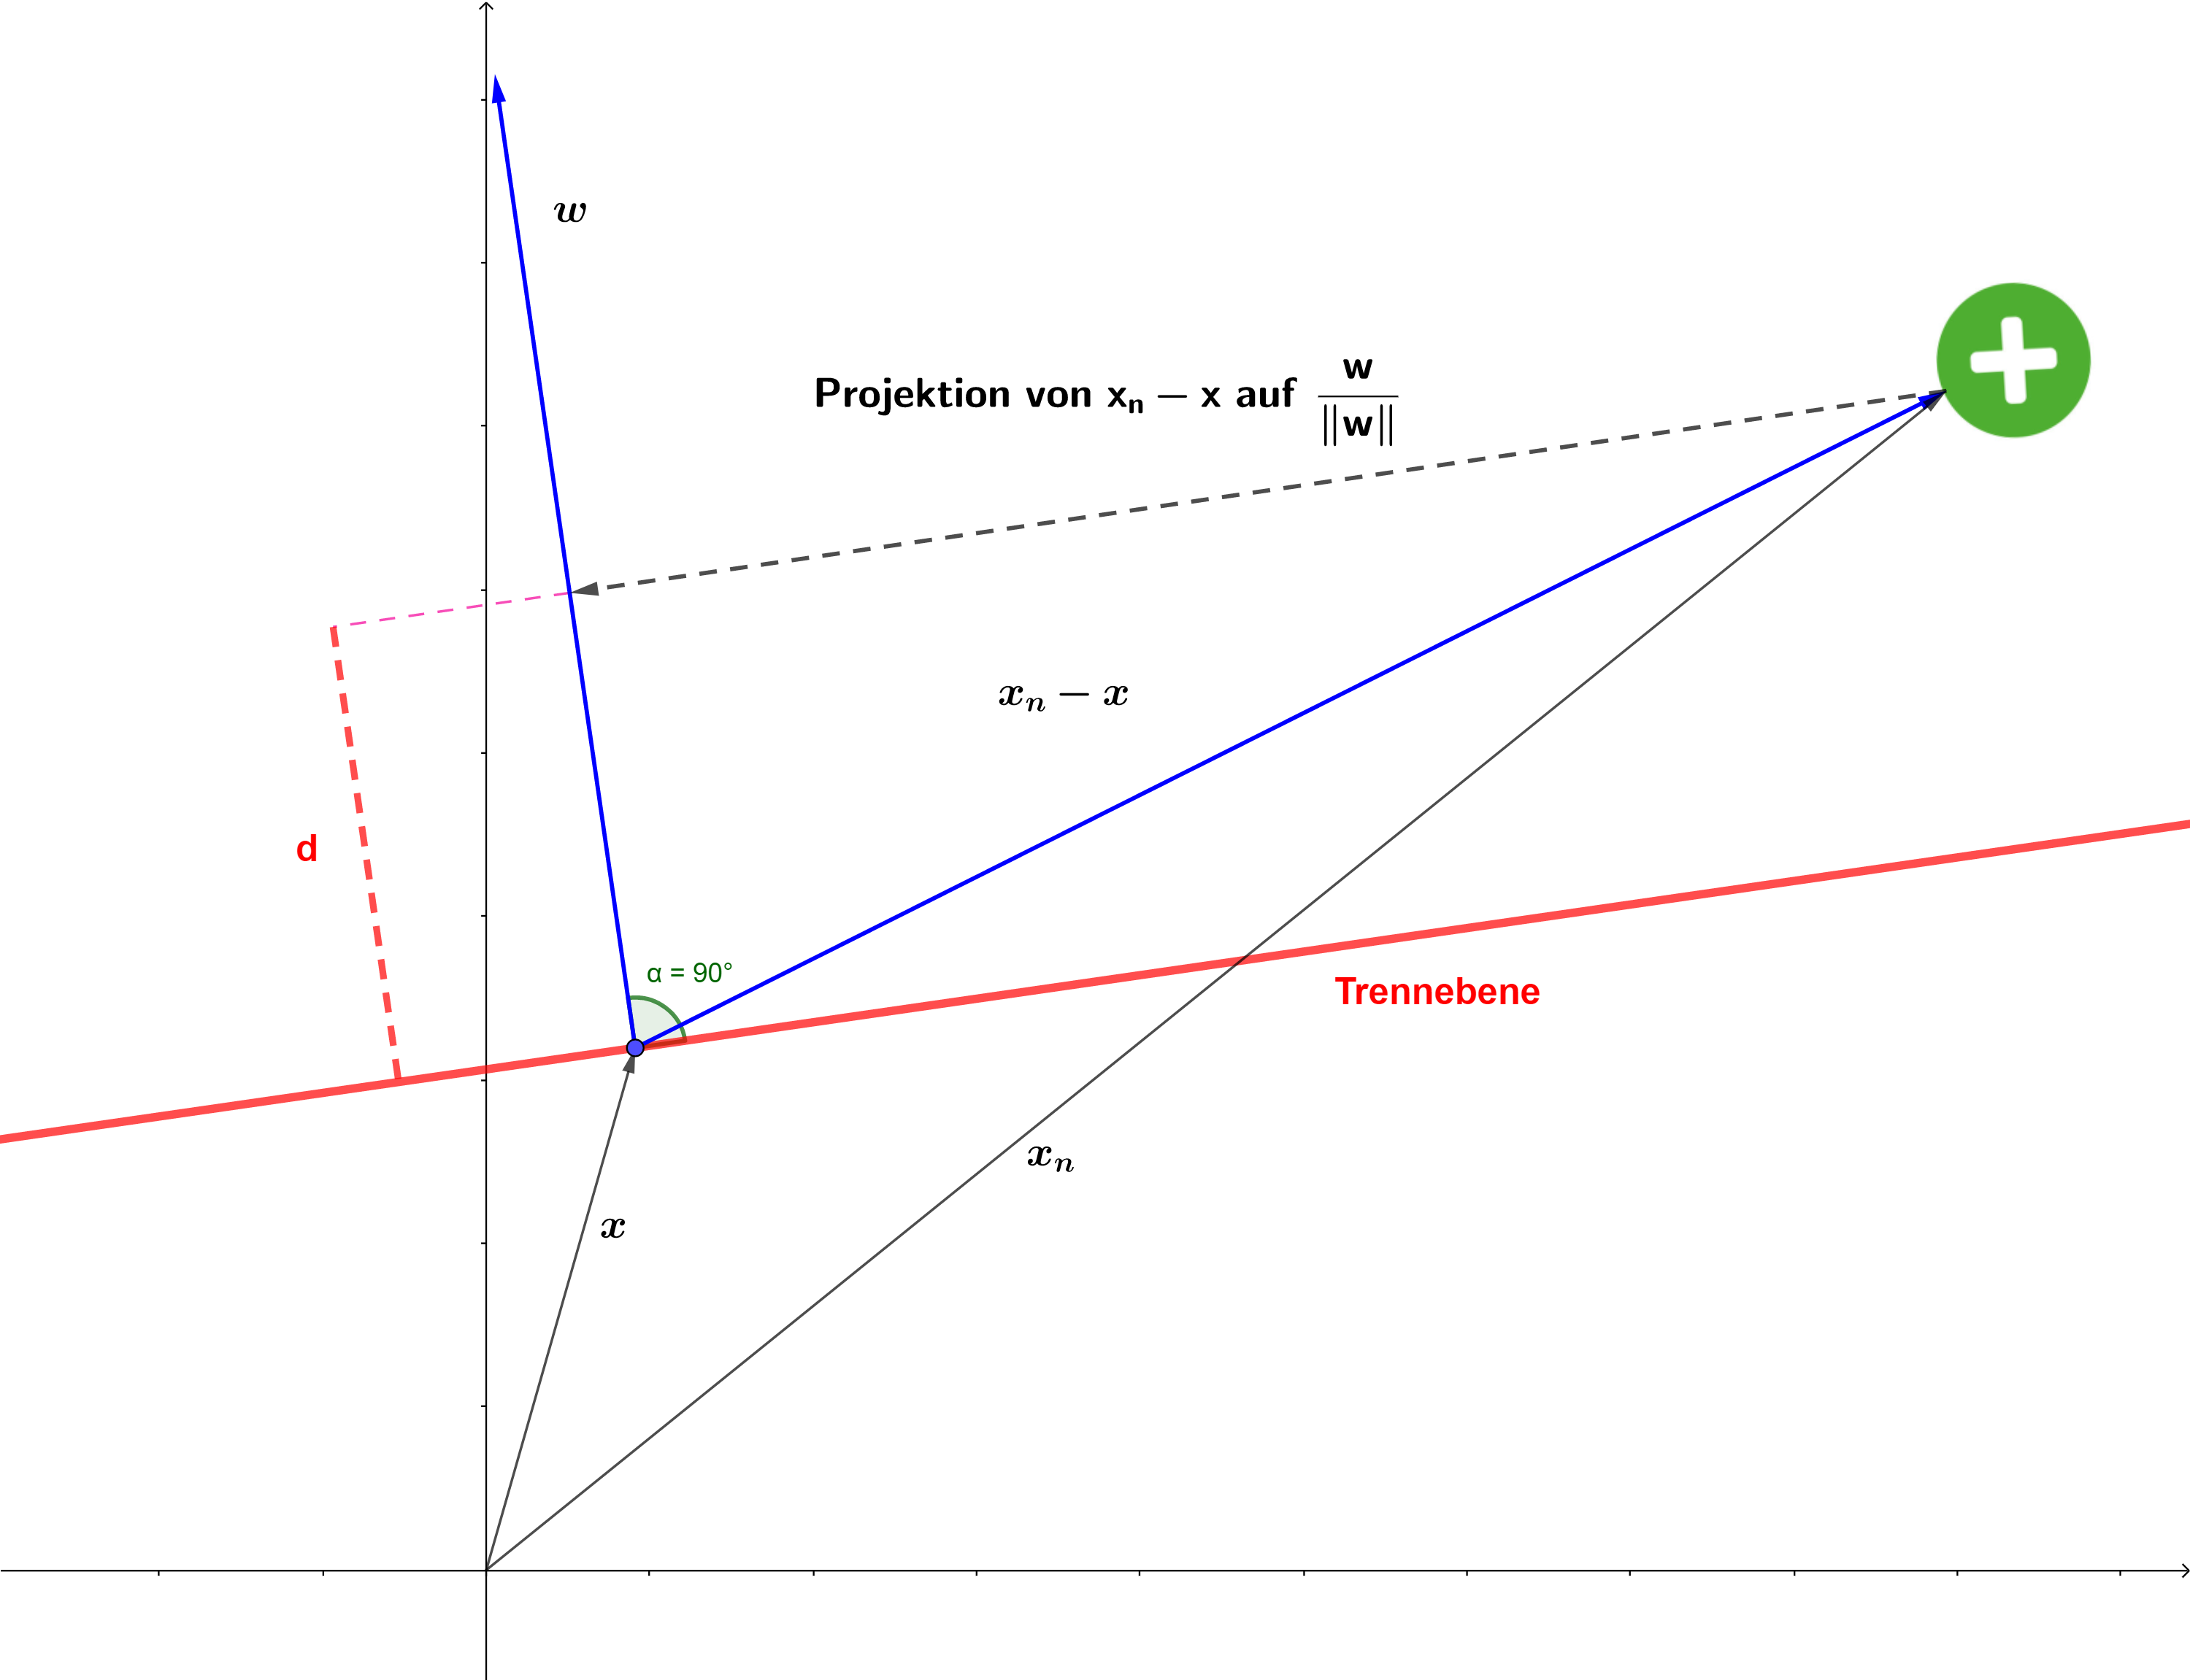
\includegraphics[width=\textwidth,height=0.8\textheight,keepaspectratio]{assets/projection.png}
		\end{figure}
	\end{center}
\end{frame}

\begin{frame}{Normalabstand eines Punktes zur Ebene}
	\begin{equation*}
		\begin{aligned}
			d &= | \frac{w^{T}}{\lVert w \rVert} (x_{n} - x) | = \\
			&= \frac{1}{\norm{w}} | (w^{T} x_{n} - w^{T} x) | =\\
			&= \frac{1}{\norm{w}} | (w^{T} x_{n} + b - (w^{T} x + b)) |
		\end{aligned}
	\end{equation*}

	\begin{center}
		\begin{figure}
			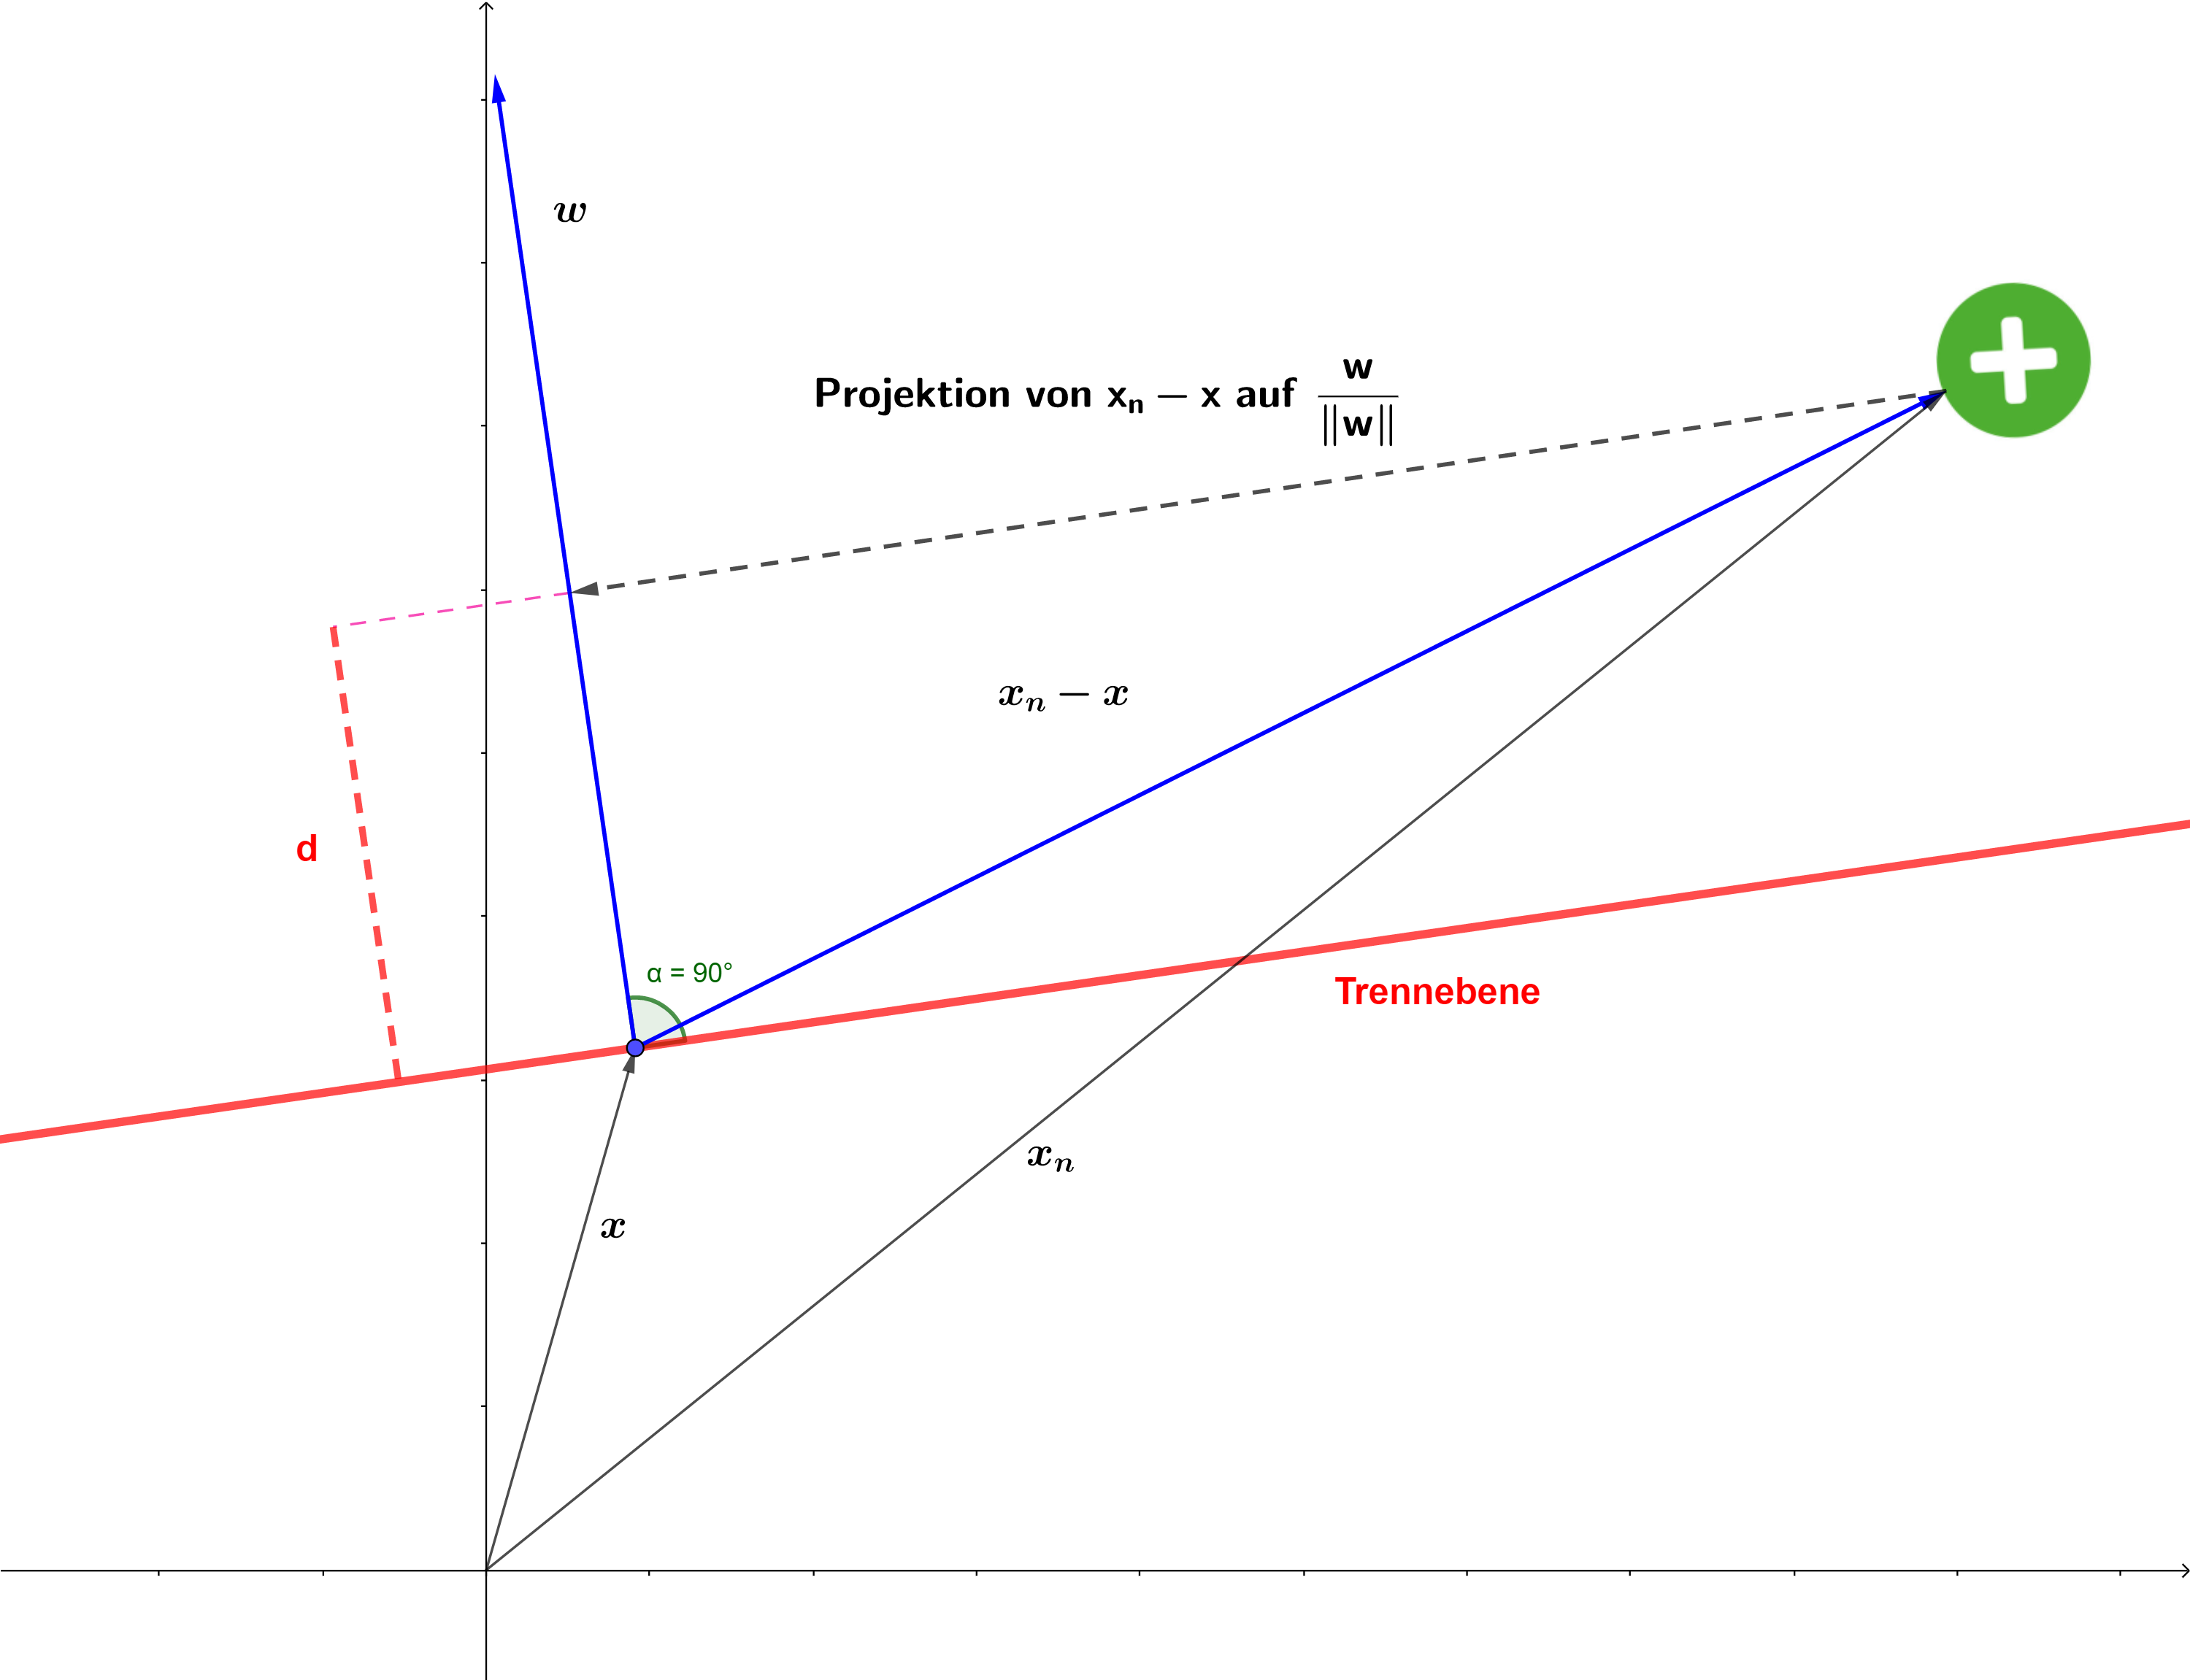
\includegraphics[width=\textwidth,height=0.5\textheight,keepaspectratio]{assets/projection.png}
		\end{figure}
	\end{center}

\end{frame}


\begin{frame}{Normalabstand eines Punktes zur Ebene}
	\begin{equation*}
		\begin{aligned}
			d &= \frac{1}{\norm{w}} | (w^{T} x_{n} + b - (w^{T} x + b)) |
		\end{aligned}
	\end{equation*}

	Weil der Punkt $x$ auf der Ebene liegt gilt $w^{T} x + b = 0$ und somit für den Normalabstand eines beliebigen Punktes $x_{n}$:
	
	\begin{equation*}
		\begin{aligned}
			d &= \frac{1}{\norm{w}} | (w^{T} x_{n} + b) |
		\end{aligned}
	\end{equation*}
\end{frame}


\begin{frame}{Breite des Trennbands}
	
	\begin{equation*}
		\begin{aligned}
			d &= \frac{1}{\norm{w}} | (w^{T} x_{n} + b) |
		\end{aligned}
	\end{equation*}

	Annahme: $x_{n} = \hat{x}$ ist der am nächsten zur Ebene liegende Punkt auf der Grenze des Trennbands\\
	Weil $y_{n} (w^{T} \hat{x} + b) = 1 = |w^{T} \hat{x} + b|$ gilt ergibt sich der minimale Normalabstand $D$: \\
	
	\begin{equation*}
		\begin{aligned}
			D &= \frac{1}{\norm{w}}
		\end{aligned}
	\end{equation*}

	 Weil $D$ der minimale Normalabstand zur Ebene ist, ist $2D$ die Breite des freien Trennbands.

\end{frame}


\begin{frame}{Reminder}
	
	Ziel: lineare Trennung mit möglichst breitem, freien Trennband \\
	
	Entspricht Maximierung:
	\begin{equation*}
		\begin{aligned}
			\max_{w} (2 D) &= \max_{w} \frac{2}{\norm{w}} = \max_{w} \frac{1}{\norm{w}}
		\end{aligned}
	\end{equation*}
	
	\begin{center}
		\begin{figure}
			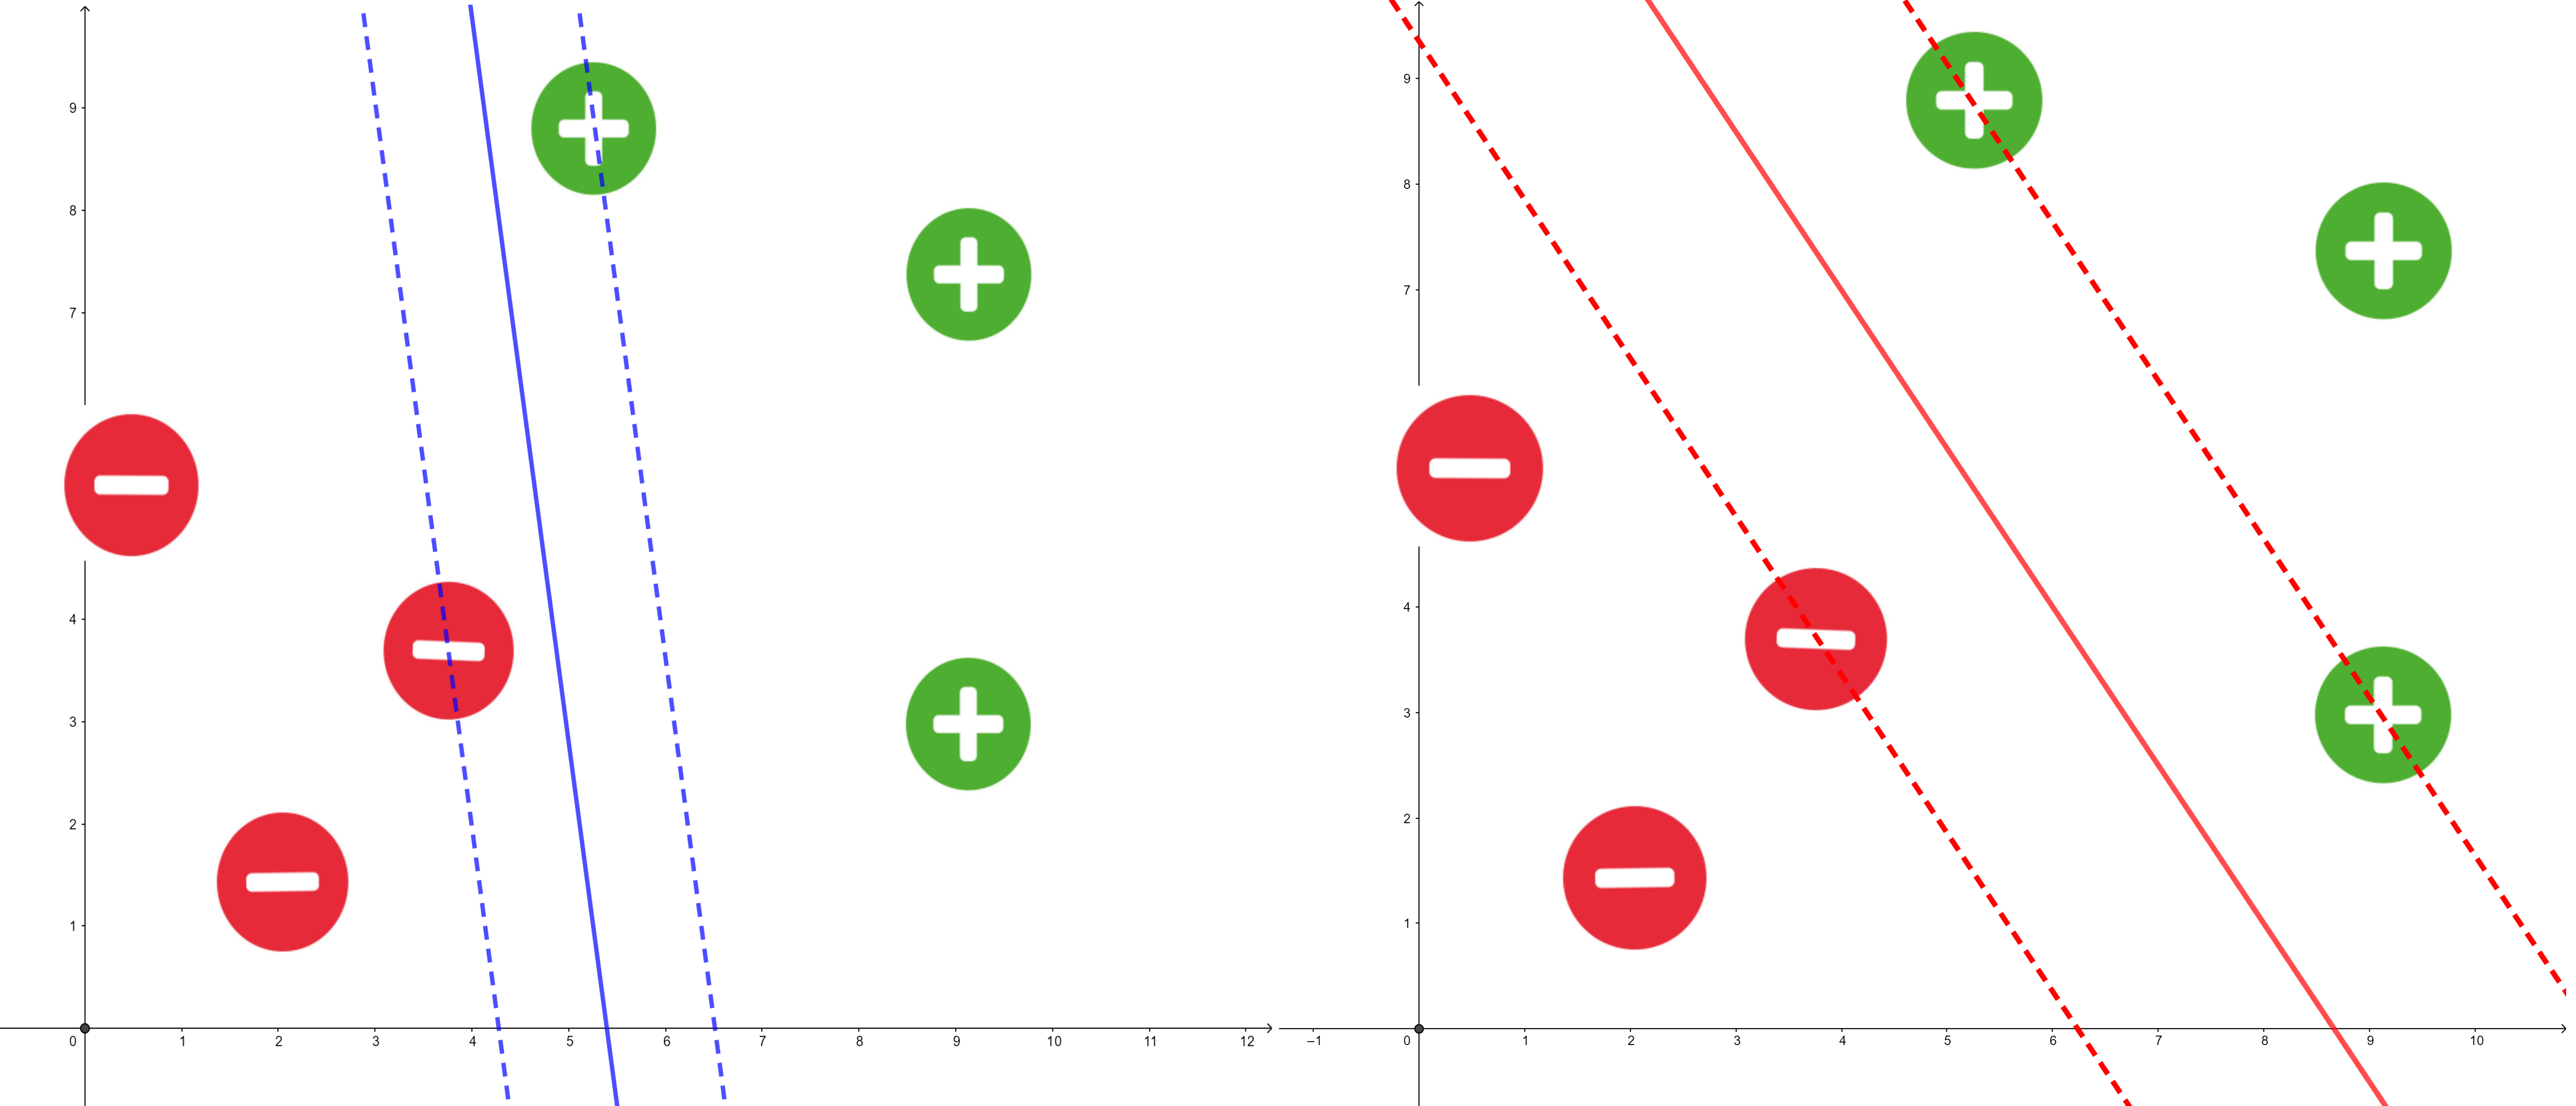
\includegraphics[width=\textwidth,height=0.7\textheight,keepaspectratio]{assets/small_vs_big_margin.png}
		\end{figure}
	\end{center}	
\end{frame}


\begin{frame}{Optimierungsproblem}
	
\begin{subequations}
	\begin{alignat*}{2}
		&\!\max_{w}        &\qquad&  \frac{1}{\norm{w}} \\
		&\text{mit } &      & \min_{n=1..N} |w^{T} x_{n} + b| = 1
	\end{alignat*}
\end{subequations}

\begin{equation*}
	\begin{aligned}
		\min_{n=1..N} |w^{T} x_{n} + b| = 1 \text{  ist der am nächsten zur Ebene liegende Punkt } \hat{x}
	\end{aligned}
\end{equation*}



Beidseitige Multiplikation mit $y_{n}$ zur Vermeidung des Betrags:
\begin{equation*}
	\begin{aligned}
		|w^{T} x_{n} + b| &= y_{n} (w^{T} x_{n} + b)
	\end{aligned}
\end{equation*}
	
\end{frame}


\begin{frame}{Optimierungsproblem}
	Nach Umformung (Maximierung in Minimierung) und Verallgemeinerung der Nebenbedingung auf beliebige Punkte $x_{n}$:
	\begin{subequations}
		\begin{alignat*}{2}
			&\!\min_{w}        &\qquad&  \frac{1}{2} w^{T} w \\
			&\text{mit } &      & y_n (w^{T} x_{n} + b) \geq 1 \text{ für } n=1..N 
		\end{alignat*}
	\end{subequations}

	Bemerkungen:
	\begin{itemize}
		\item Faktor $\frac{1}{2}$ wird so gewählt weil dieser später wegfällt
		\item $w^{T} w $ und $\norm{w}$ sind aus Optimierungssicht gleichbedeutend, Problem ist in dieser Form aber besser optimierbar
	\end{itemize}

\end{frame}

\begin{frame}{Lagrange Optimierung}
	Optimierungsproblem mit Ungleichung als Nebenbedingung \\
	Umformen der Nebenbedingung:
	\begin{subequations}
		\begin{alignat*}{2}
			&\!\min_{w}        &\qquad&  \frac{1}{2} w^{T} w\\
			&\text{mit } &      & y_n (w^{T} x_{n} + b)-1 \geq 0 \text{ für } n=1..N
		\end{alignat*}
	\end{subequations}
\end{frame}

\begin{frame}{Aufstellen der Lagrange Gleichung}
	Ungleichung wird von zu optimierender Funktion abgezogen und Lagrange Multiplikatoren eingeführt:
	\begin{subequations}
		\begin{alignat*}{2}
			&\!\min_{w, b}        &\qquad&  \Lagr (w, b, \alpha) = \frac{1}{2} w^{T} w - \sum_{n=1}^{N} \alpha_{n} (y_n (w^{T} x_{n} + b)-1)\\
			&\max_{\alpha_{n}} &      & \alpha_{n} \geq 0 \text{ für } n=1..N
		\end{alignat*}
	\end{subequations}

	Lösung durch $0$ setzen der partiellen Ableitungen:
	\begin{equation*}
		\begin{aligned}
			\nabla_{w} \Lagr &\overset{!}{=} \vec{0} \\
			\frac{\partial}{\partial b} \Lagr &\overset{!}{=} 0 \\
		\end{aligned}
	\end{equation*}
	
\end{frame}

\begin{frame}{Lösen der Lagrange Gleichung}

	Nach $w$:
	\begin{equation*}
		\begin{aligned}
			\nabla_{w} \Lagr &= w - \sum_{n=1}^{N} \alpha_{n} y_{n} x_{n} \overset{!}{=} \vec{0} \\
			w &= \sum_{n=1}^{N} \alpha_{n} y_{n} x_{n}
		\end{aligned}
	\end{equation*}

	Nach $b$:
	\begin{equation*}
		\begin{aligned}
			\frac{\partial}{\partial b} \Lagr &= - \sum_{n=1}^{N} \alpha_{n} y_{n} \overset{!}{=} 0 \\
			\sum_{n=1}^{N} \alpha_{n} y_{n} &= 0
		\end{aligned}
	\end{equation*}
\end{frame}

\begin{frame}{Rücksubstitution in Lagrange Gleichung}
Aufteilen der Summe:
\begin{equation*}
	\begin{aligned}
		\Lagr(w, b, \alpha) &= \frac{1}{2} w^{T} w - \sum_{n=1}^{N} \alpha_{n} (y_n (w^{T} x_{n} + b)-1) = \\
		&= \frac{1}{2} w^{T} w - [\sum_{n=1}^{N} \alpha_{n} y_{n} b - \sum_{n=1}^{N} \alpha_{n} + \sum_{n=1}^{N} \alpha_{n} y_{n} w^{T} x_{n}]
	\end{aligned}
\end{equation*}

Aus Ableitung nach $b$ wissen wir $\sum_{n=1}^{N} \alpha_{n} y_{n} = 0$:

\begin{equation*}
	\begin{aligned}
		\Lagr(w, b, \alpha) &= \frac{1}{2} w^{T} w - [-\sum_{n=1}^{N} \alpha_{n} + \sum_{n=1}^{N} \alpha_{n} y_{n} w^{T} x_{n}]
	\end{aligned}
\end{equation*}

\end{frame}


\begin{frame}{Rücksubstitution in Lagrange Gleichung}
Vergleicht man den Term $\sum_{n=1}^{N} \alpha_{n} y_{n} w^{T} x_{n}$ mit dem Ergebnis der partiellen Ableitung nach $w$ ($w = \sum_{n=1}^{N} \alpha_{n} y_{n} x_{n}$) erkennt man, dass gilt:

\begin{equation*}
	\begin{aligned}
		\sum_{n=1}^{N} \alpha_{n} y_{n} w^{T} x_{n} &= w^T w = \\
		&= \sum_{n=1}^{N} \sum_{m=1}^{M} y_{n} y_{m} \alpha_{n} \alpha_{m} x_{n}^{T} x_{m}
	\end{aligned}
\end{equation*}

Eingesetzt in Lagrange Gleichung:
\begin{equation*}
	\begin{aligned}
		\Lagr(\alpha) &= \sum_{n=1}^{N }\alpha_{n} - \frac{1}{2} \sum_{n=1}^{N} \sum_{m=1}^{M} y_{n} y_{m} \alpha_{n} \alpha_{m} x_{n}^{T} x_{m}
	\end{aligned}
\end{equation*}

\end{frame}


\begin{frame}{Maximierung ohne Nebenbedingung}
	Quadratic Programming Problem ($x_{n}^{T} x_{m}$):
	\begin{subequations}
		\begin{alignat*}{2}
			&\!\max_{\alpha}        &\qquad&  	\Lagr(\alpha) = \sum_{n=1}^{N} \alpha_{n} - \frac{1}{2} \sum_{n=1}^{N} \sum_{m=1}^{M} y_{n} y_{m} \alpha_{n} \alpha_{m} x_{n}^{T} x_{m}\\
			&\text{mit } &      & \alpha_{n} \geq 0 \text{ für } n=1..N \\
			&       & & \sum_{n=1}^{N} \alpha_{n} y_{n} = 0\text{ für } n=1..N
		\end{alignat*}
	\end{subequations}

	Lösung mittels QP-Solver \\
	Ergebnis: $\alpha$ Vektor mit $\alpha_{n}$ Lagrange-Multiplikatoren

\end{frame}


\begin{frame}{Schlupfterm}
	Reminder Ausgangsproblem:
	\begin{subequations}
		\begin{alignat*}{2}
			&\!\min_{w, b}        &\qquad&  \Lagr (w, b, \alpha) = \frac{1}{2} w^{T} w - \sum_{n=1}^{N} \alpha_{n} (y_n (w^{T} x_{n} + b)-1)\\
			&\max_{\alpha_{n}} &      & \alpha_{n} \geq 0 \text{ für } n=1..N
		\end{alignat*}
	\end{subequations}
	
	
	 $\alpha_{n} (y_n (w^{T} x_{n} + b)-1)$ (\glqq Schlupf \grqq) wird $0$ wenn:
	 \begin{itemize}
	 	\item $\alpha_{n} = 0$ oder 
	 	\item $(y_n (w^{T} x_{n} + b)-1) = 0$
	 \end{itemize}
	 
	 Umgekehrt: Alle $x_{n}$ mit $\alpha_{n} \neq 0$ haben Schlupf $0$, liegen also am nächsten zur Trennebene. \\
	 
	 Diese Vektoren werden \textbf{Stützvektoren} genannt.
\end{frame}

\begin{frame}{Bestimmung Gewichtsvektor}
	
	$\alpha$ Vektor mit $\alpha_{n}$ Faktoren ist bekannt aus QP-Solver\\
	Viele $\alpha_{i}$ werden $0$ sein, die $\alpha_{i} \neq 0$ gehören zu den Stützvektoren $x_{i}$. \\
	Damit kann Formel für $w$
	\begin{equation*}
		\begin{aligned}
			w &= \sum_{n=1}^{N} \alpha_{n} y_{n} x_{n}
		\end{aligned}
	\end{equation*}

	vereinfacht werden:
	\begin{equation*}
	\begin{aligned}
		w &= \sum_{n \text{ ist Sützvektor}} \alpha_{n} y_{n} x_{n}
	\end{aligned}
	\end{equation*}

	Die Bezeichnung Stützvektor ergibt sich, weil die Ebene durch diese Vektoren \glqq gestützt \grqq wird. Alle Vektoren mit $\alpha_{n} = 0$ haben keinen Einfluss!
\end{frame}

\begin{frame}{Bestimmung Bias}
	
	$y_n (w^{T} x_{n} + b) = 1$ gilt für Stützvektoren, daher kann mit beliebigem Stützvektor $x_{n}$ der Bias bestimmt werden:
	
	\begin{equation*}
		\begin{aligned}
			b &= \frac{1}{y_{n}} - w^{T} x_{n} = \\
			&= y_{n} - w^{T} x_{n} 
		\end{aligned}
	\end{equation*}
	
	
\end{frame}


\section{Lösung mittels QP-Solver}

\begin{frame}{Lösung mittels QP-Solver}
	
	Standardform von QP-Problemen:
	\begin{equation*} \label{std_QP_problem}
		\begin{aligned}
			\min_{x} &= \frac{1}{2} x^{T} Q x + c x + d 
		\end{aligned}
	\end{equation*}
	
	Umformung Maximierung in Minimierung weil $\max -f(x) = \min f(x)$:
	\begin{equation*} \label{qp_adapt1}
		\begin{aligned}
			\min_{\alpha} \Lagr(\alpha) &= \frac{1}{2} \sum_{n=1}^{N} \sum_{m=1}^{M} y_{n} y_{m} \alpha_{n} \alpha_{m} x_{n}^{T} x_{m} - \sum_{n=1}^{N} \alpha_{n}
		\end{aligned}
	\end{equation*}
\end{frame}

\begin{frame}{Problem in QP-Standardform}
	
	\begin{equation*}
		\begin{aligned}
			\min_{\alpha} \Lagr(\alpha) &= \frac{1}{2} \sum_{n=1}^{N} \sum_{m=1}^{M} y_{n} y_{m} \alpha_{n} \alpha_{m} x_{n}^{T} x_{m} - \sum_{n=1}^{N} \alpha_{n}
		\end{aligned}
	\end{equation*}
	
	In QP-Standardform $\rightarrow$ Lösungs-Frameworks:
	
	\begin{subequations}
		\begin{alignat*}{2}
			&\!\min_{\alpha}        &\qquad& \Lagr(\alpha) = \frac{1}{2} \alpha^{T} Q \alpha + (-1^T) \alpha \label{eq:qp1}\\
			&\text{mit} &      & Q = \begin{bmatrix} 
				y_{1}y_{1}x_{1}^{T}x_{1} & y_{1}y_{2}x_{1}^{T}x_{2} & \dots & y_{1}y_{N}x_{1}^{T}x_{N}\\
				y_{2}y_{1}x_{2}^{T}x_{1} & y_{2}y_{2}x_{2}^{T}x_{2} & \dots & y_{2}y_{N}x_{2}^{T}x_{N}\\
				\vdots & \vdots & \vdots & \vdots\\
				y_{N}y_{1}x_{N}^{T}x_{1} & y_{N}y_{2}x_{N}^{T}x_{2} & \dots & y_{N}y_{N}x_{N}^{T}x_{N}\\ 
			\end{bmatrix}
		\end{alignat*}
	\end{subequations}

	\pause

	$Q$ ist $N \times N$ Matrix. Problematisch bei großen Trainingssets!
\end{frame}

\begin{frame}{Lösung mittels QP-Solver}
	Ergebnis des QP-Solvers: $\alpha = (\alpha_{1}, \alpha_{2}, ..., \alpha_{n})$ \\
	
	Berechnung von $w$ und $b$ wie zuvor gezeigt:
	
	\begin{equation*}
		\begin{aligned}
			w &= \sum_{n=1}^{N} \alpha_{n} y_{n} x_{n}
		\end{aligned}
	\end{equation*}

	Mit beliebigem Stützvektor $x_{k}$:
	\begin{equation*}
		\begin{aligned}
			b &= \frac{1}{y_{k}} - w^{T} x_{k}
		\end{aligned}
	\end{equation*}

	Klassifikation neuer Eingaben $x$:
	\begin{equation*}
		\begin{aligned}
			y &= sign(w^{T} x + b)
		\end{aligned}
	\end{equation*}

\end{frame}







\begin{frame} {A test with images}
	\framesubtitle{subcaption testing with images}
	\begin{minipage}{0.5\textwidth}

		\begin{itemize}
			\item Some 
			\item text 
			\item on left side of slide here..
			\item \cref{fig:intuition_margin} zeigt blabla.
		\end{itemize}
		\pause
	\end{minipage} \hfill
	\begin{minipage}{0.45\textwidth}
	\begin{figure}
		\centering
		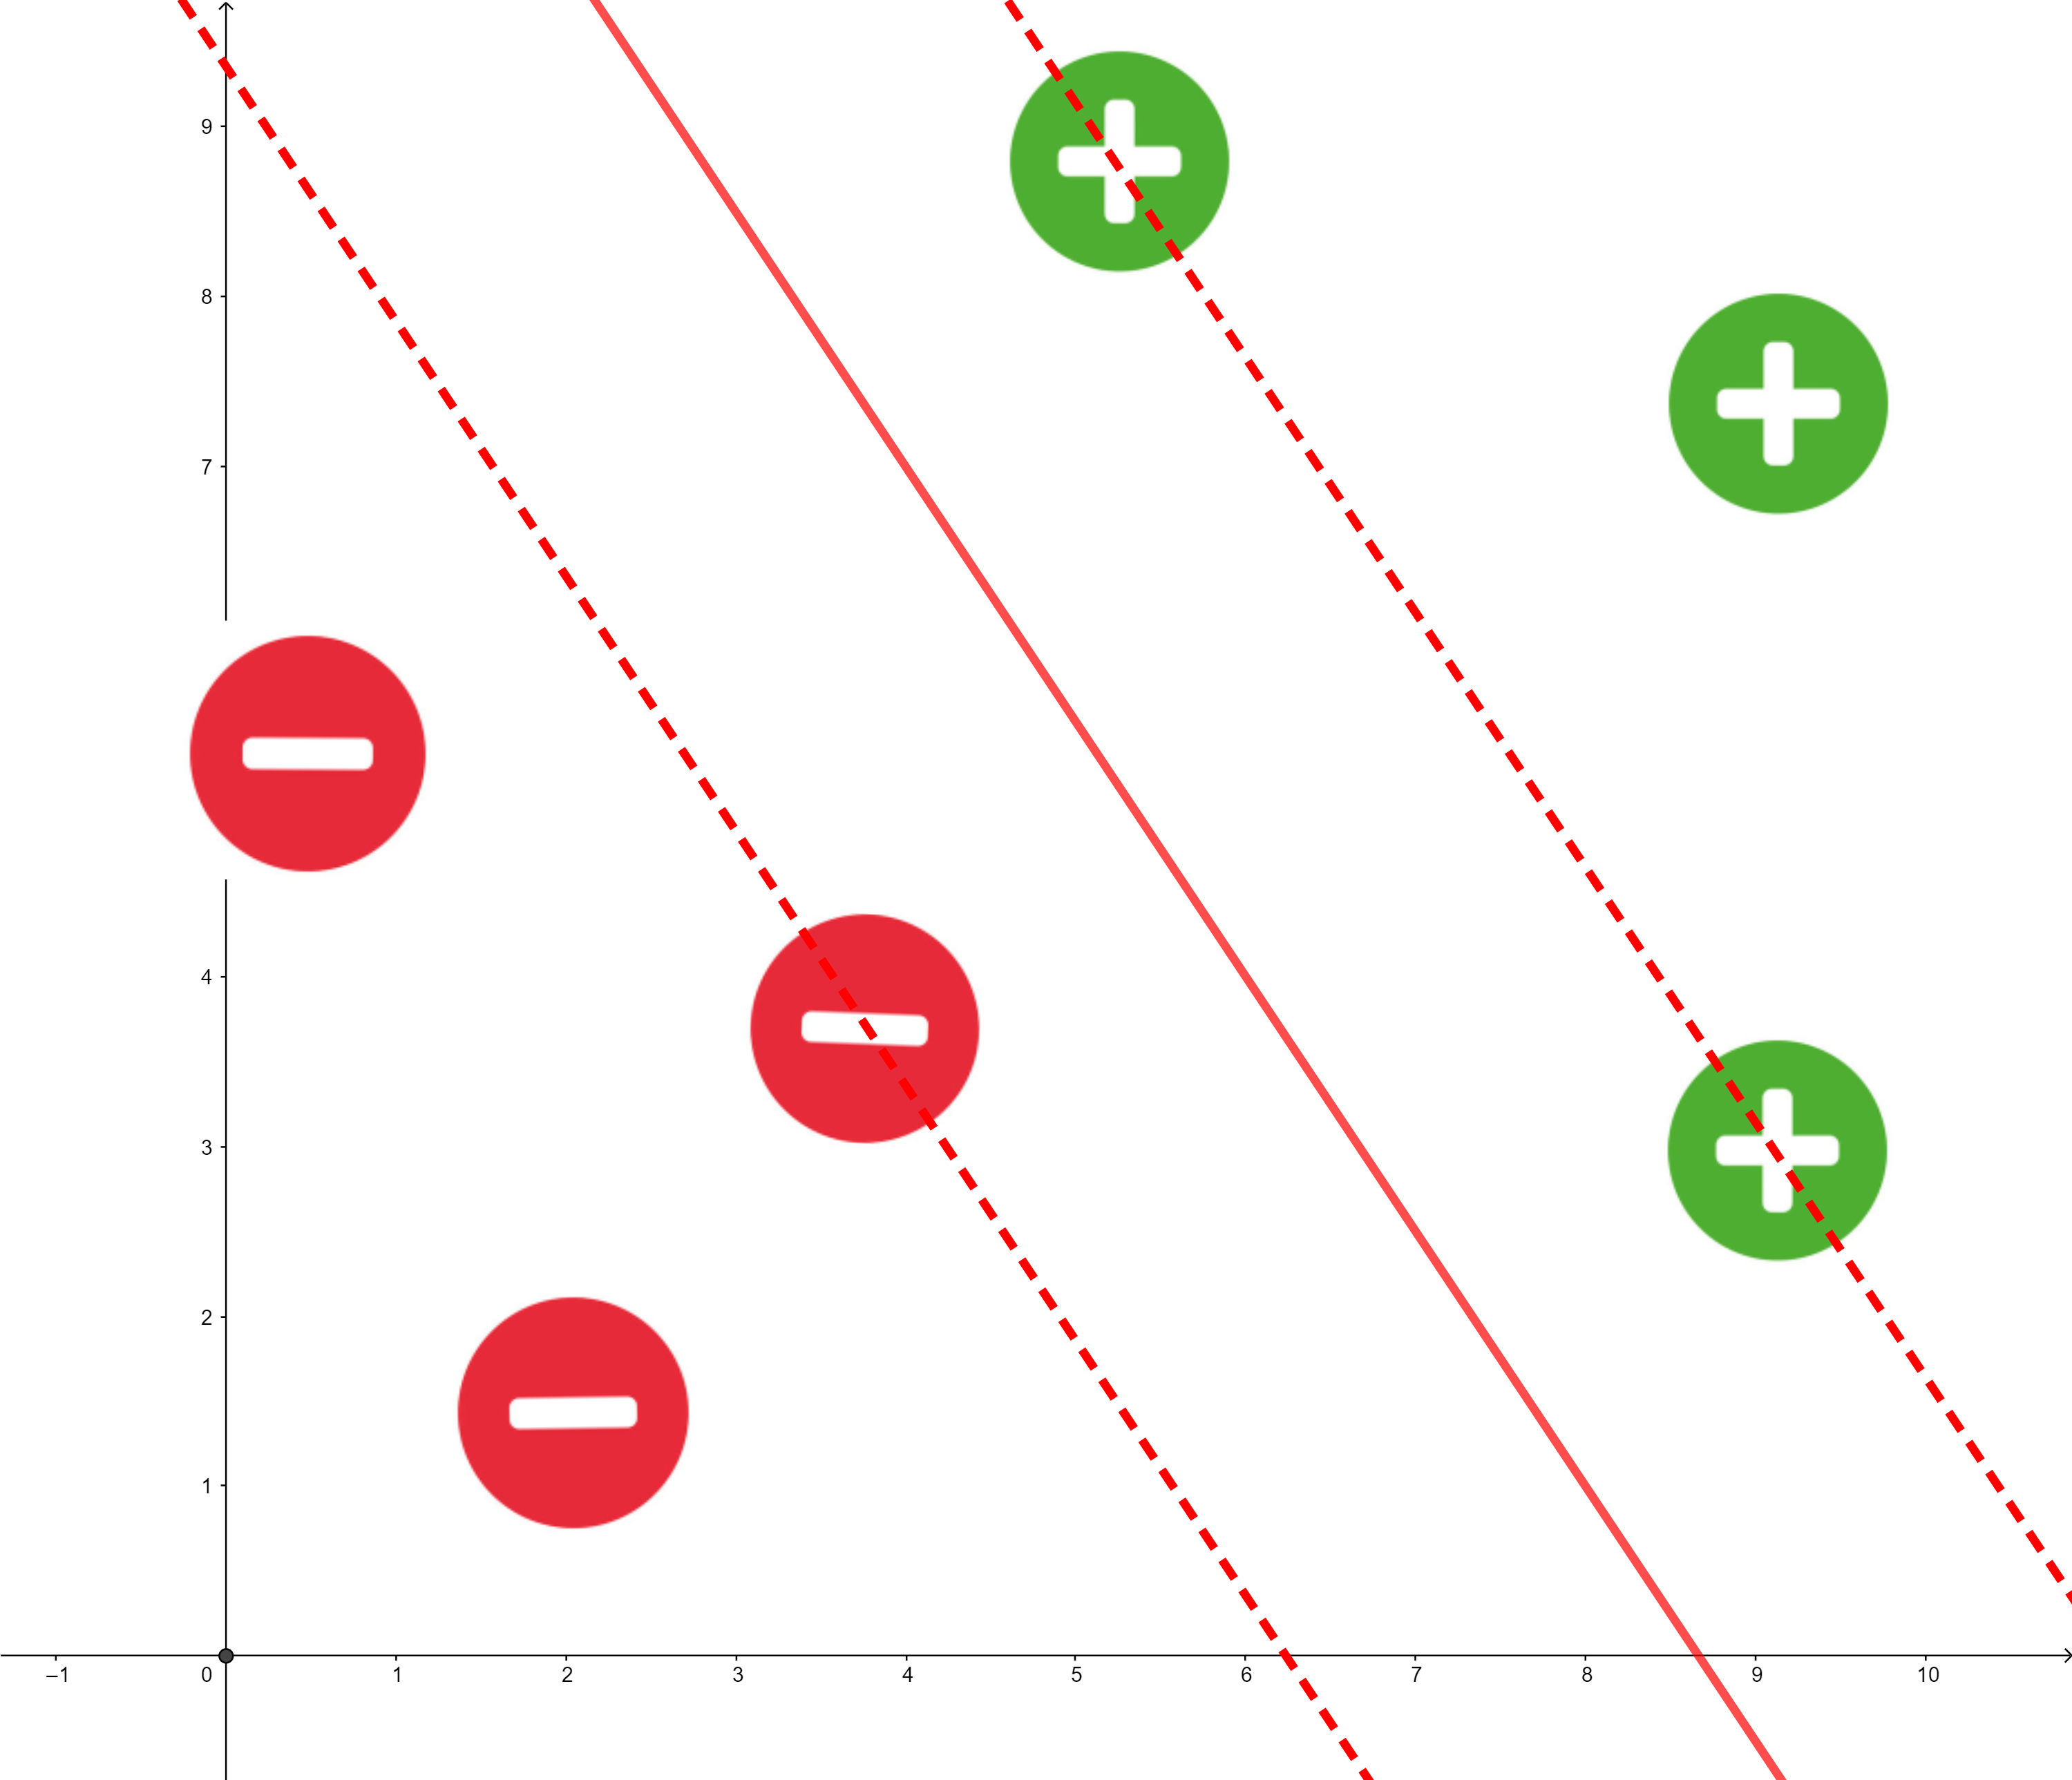
\includegraphics[height=0.9\textwidth]{assets/intuition_big_margin.png}
		\caption{Abhängig von der Lage der Trennebene entstehen schmale (blau) oder breite (rot) Trennbänder. Ziel ist die Maximierung der Breite des Trennbands durch die Ermittlung der optimalen Lage der Trennebene.}
		\label{fig:intuition_margin}
	\end{figure}
	\end{minipage}
\end{frame}

\begin{frame}{citation tests}
	\begin{subequations} \label{svm_classify1}
		\begin{alignat}{2}
			y = sign(w^{T} x + b)  & \qquad & \text{ gleichbedeutend mit} \\
			w^{T} x + b > 0 & & \text{ für } y = +1\\
			w^{T} x + b < 0 & & \text{ für } y = -1
		\end{alignat}
	\end{subequations}

	In \cref{svm_classify1} wird .. \\
	
	Footcite example \footcite{platt_sequential_1998} \\
	
	\textcite{burges_tutorial_1998}
\end{frame}


\section{Soft-Margin Support Vector Machine}

\section{Vergleich Hard- \& Soft-Margin Support Vector Machine}

\section{Nichtlineare Trennung}



\begin{frame}[standout]
	Fragen?
\end{frame}

\begin{frame}
	\printbibliography
\end{frame}



\end{document}



